\chapter{Coleta de informações sobre a instituição} \label{chap:instituicao} % ## 4

% Como citado pelos autores [FAZER REFERÊNCIA À TODOS OS AUTORES QUE FALAM DISSO], o
O problema de criação de grade horária tem forte influência da estrutura organizacional da instituição. Por tal motivo, este capítulo tem como objetivo apresentar a estrutura organizacional da \LinkToURL{\LinkSiteUENF}{Universidade Estadual do Norte Fluminense Darcy Ribeiro (UENF)} e como se dá o processo de criação de grades horárias na mesma. Essa apresentação se mostra necessária para que se possa entender melhor o problema e as possíveis soluções.

A apresentação se dará em três partes principais: a explanação sobre \hyperref[sec:estatuto]{como a UENF está definida segundo seus documentos oficiais}, a análise qualitativa das \hyperref[sec:entrevistas]{entrevistas realizadas com os principais envolvidos no processo de criação de grades horárias} e a análise quantitativa das respostas do \hyperref[sec:formulario]{questionário aplicado aos alunos da UENF}. Os dois primeiros tópicos convergem na criação de uma \hyperref[sec:sequencia]{sequência de criação de grades horárias}. Por fim, será apresentada a análise das \hyperref[sec:relacoes]{relações entre as variáveis} envolvidas no processo de criação de grades horárias.

% Vindo da introdução:
% Essas informações serão relevantes para se atingir a satisfação e uso futuro do sistema proposto.
% Espera-se com este capítulo fornecer um entendimento amplo e, ao mesmo tempo, focalizado o bastante, para que se possa compreender claramente o processo de criação de grades horárias na UENF e os fatores que o influenciam.

\section{A UENF} \label{sec:estatuto} % ### 4.1

A UENF conta com diversos documentos que visam regulamentar e explicar seu funcionamento. Os documentos vão desde o mais alto nível onde se atribui as funções da UENF, até o menor nível onde se mostra a Grade Curricular para o curso de Ciência da Computação. Desses documentos, podemos listar o Estatuto da UENF \cite{Estatuto2002}, o Plano de Desenvolvimento Institucional \cite{PDI2023}, o Regimento Geral da UENF \cite{RegimentoGeralUENF2006}, o Regimento Geral da Graduação \cite{RegimentoGeralGraduação2012}, o Regimento da Câmara de Graduação \cite{RegimentoCâmaraGraduação2012}, as Normas da Graduação \cite{Normas2012}, os Projetos Pedagógicos do Curso de Ciência da Computação \cite{PPCCC2005, PPCCC2015, PPCCC2022} e a Matriz Curricular do Curso de Ciência da Computação \cite{Matriz2015}.

% Provavelmente eu deveria adicionar informações sobre a secretaria acadêmica
% Precisa de revisão
% Sinto que falta falar sobre secretaria acadêmica e Conselho de Centro

Segundo o estatuto, a UENF compreende os \textbf{Órgãos da Administração Superior de política, gestão e supervisão}; \textbf{Unidades universitárias de ensino, pesquisa e extensão}; e os \textbf{Órgãos e serviços especiais, destinados a auxiliar na administração e a suplementar as atividades de ensino, pesquisa, extensão e apoio técnico}.

Quanto aos órgãos da Administração Superior devemos enfocar o órgão executivo, constituído unicamente pela reitoria, cujos órgãos auxiliares englobam a Secretaria Acadêmica, que por sua vez tem como algumas de suas atribuições as seguintes: Coordenar a \textbf{divulgação do horário escolar dos vários cursos da UENF}, de modo a \textbf{otimizar os recursos humanos}, \textbf{ampliar as opções de disciplinas para os alunos} e tornar acessíveis os dados escolares; e \textbf{Centralizar os serviços de registro da vida escolar dos alunos}, compreendendo \textbf{inscrição}, admissão, \textbf{matrícula}, \textbf{créditos}, \textbf{opções}, transferências, promoções, graduações e preparação dos respectivos diplomas, dentro das normas estabelecidas.

Já quanto as unidades universitárias de ensino, temos no estatuto que ``as unidades universitárias de ensino, pesquisa e extensão, definidas por áreas de conhecimento, são constituídas em Centros, que por sua vez congregam Laboratórios afins'' e que ``o Laboratório é a menor parte da estrutura universitária para todos os efeitos de organização administrativa, didático-científica, distribuição de pessoal e de representação nos órgãos colegiados da UENF''.

A administração do Centro é da competência do Diretor e seu Conselho. Os Laboratórios, por sua vez, são administrados pelos Chefes de Laboratório.

O Conselho de Centro, tem como uma de suas atribuições, descrito no inciso XVII do artigo 34 do estatuto, a seguinte: \textbf{designar, semestralmente, os professores responsáveis pelas disciplinas dos Cursos de Graduação} e Programas de Pós-Graduação, ouvidos os respectivos Laboratórios, os Colegiados de Curso e Comissões de Coordenação. Atualmente, segundo o site da UENF, a universidade possui 4 Centros, sendo eles: Centro de Ciências do Homem - \LinkToURL{\LinkCCH}{CCH}; Centro de Ciência e Tecnologia - \LinkToURL{\LinkCCT}{CCT}; Centro de Biociências e Biotecnologia - \LinkToURL{\LinkCBB}{CBB}; Centro de Ciências e Tecnologias Agropecuárias - \LinkToURL{\LinkCCTA}{CCTA}.

E também existem 8 \LinkToURL{\LinkLaboratorios}{laboratórios} vinculados ao Centro de Ciência e Tecnologia (CCT), sendo eles:

\begin{enumerate}[nosep]
  \item Laboratório de Meteorologia – \LinkToURL{\LinkLAMET}{LAMET};
  \item Laboratório de Ciências Físicas – \LinkToURL{\LinkLCFIS}{LCFIS};
  \item Laboratório de Engenharia Civil – \LinkToURL{\LinkLECIV}{LECIV};
  \item Laboratório de Ciências Químicas – \LinkToURL{\LinkLCQUI}{LCQUI};
  \item Laboratório de Materiais Avançados – \LinkToURL{\LinkLAMAV}{LAMAV};
  \item Laboratório de Ciências Matemáticas – \LinkToURL{\LinkLCMAT}{LCMAT};
  \item Laboratório de Engenharia de Produção – \LinkToURL{\LinkLEPROD}{LEPROD};
  \item Laboratório de Engenharia e Exploração de Petróleo – \LinkToURL{\LinkLENEP}{LENEP}.
\end{enumerate}

Os Laboratórios englobam os Cursos de Graduação e Pós-Graduação, que são administrados pelos Coordenadores de Curso. Além disso, o LCMAT mantém dois cursos de graduação e um programa de pós-graduação stricto sensu. Sendo eles:

\begin{enumerate}[nosep]
  \item \LinkToURL{\LinkLicMat}{Licenciatura em Matemática};
  \item \LinkToURL{\LinkSiteCCUENF}{Bacharelado em Ciência da Computação};
  \item \LinkToURL{\LinkLCMATPósGraduação}{Mestrado Profissional em Matemática} – \LinkToURL{\LinkUENFPósGraduações}{PROFMAT} / \LinkToURL{\LinkProfMat}{SBM}.
\end{enumerate}

\subsection{Responsáveis pela criação das grades horárias} \label{ssec:responsaveis} % #### 4.1.1

As atribuições de cada setor estão, em sua maioria, descritas nas documentações encontradas. De forma resumida suas as atribuições são:

\begin{itemize}
  \item \textbf{Secretaria Acadêmica}: elaborar e divulgar o Calendário Acadêmico; otimizar os recursos humanos; ampliar a oferta de disciplinas;
  \item \textbf{Câmara de Graduação}: aprovar e modificar o calendário acadêmico; sugerir vagas de bolsistas;
  \item \textbf{Direção de Centro}: designação semestral de professores responsáveis pelas disciplinas, após ouvir os Laboratórios, Colegiados e Coordenações;
  \item \textbf{Chefia do Laboratório}: atribuir carga horária didática aos docentes do laboratório e aos bolsistas; designar docente responsável por disciplina ofertada;
  \item \textbf{Coordenação do Curso}: coordenar a distribuição de estudantes do curso; indicar à chefia de laboratório as disciplinas a serem ofertadas ao curso coordenado;
  \item \textbf{Sistema Acadêmico}: articula parcialmente as informações entre os setores, como a oferta de disciplinas e a distribuição de estudantes.
\end{itemize}

\section{Entrevistas} \label{sec:entrevistas} % ### 4.2

% Separar entrevistas de minhas opiniões pessoais

Como forma de entender melhor a percepção real daqueles que recorrentemente lidam com a tarefa de criação da grade horária, diversas entrevistas foram feitas com o intuito de analisar qualitativamente quais são as opiniões, pedidos, reclamações e pensamentos de diferentes níveis organizacionais da UENF. Essas análises têm como objetivo principal averiguar se o processo de criação de grades horárias realizada na UENF se apresenta como uma tarefa problemática e se a solução proposta neste trabalho se mostra como uma solução viável.

Pois, como é informado por \citeonline{PierreSWEBOK2014}, uma das fontes de requisitos é o ambiente organizacional e como o \textit{software} muitas vezes visa auxiliar em algum processo da instituição, processo este já condicionado à sua estrutura, cultura e políticas externas, o engenheiro de \textit{software} precisa estar atento a elas, visto que o novo \textit{software} não deve forçar mudanças não planejadas em processos de negócios.

\subsection{Direção do CCT} \label{ssec:3_Diretor} % #### 4.2.1

O primeiro entrevistado, em 7 de agosto de 2023, foi o Diretor do CCT. Ele atualmente estrutura a relação de disciplinas ofertadas pelo CCT em Excel e as publica \LinkToURL{\LinkDistribuiçãoDeSalas}{em formato PDF no site do CCT}. Seu trabalho auxilia os Chefes de Laboratório e Coordenadores de Curso a visualizarem quais são as salas disponíveis e em quais horários cada professor está alocado.

Um dos tópicos dialogados, foi quanto às categorias das disciplinas, ou seja, quais características notáveis as disciplinas poderiam ter. Com isso podemos listar as seguintes categorias de disciplinas:

\begin{itemize}[nosep]
  \item \textbf{Anuais}: disciplinas que ocorrem apenas uma vez no ano;
  \item \textbf{Ímpares}: disciplinas que são ofertadas no primeiro semestre letivo;
  \item \textbf{Pares}: disciplinas que são ofertadas no segundo semestre letivo;
  \item \textbf{De serviço}: disciplinas ofertadas para mais de um curso simultaneamente;
  \item \textbf{Ciclo básico}: disciplinas oferecidas para todas as engenharias;
  \item \textbf{Repetentes}: turmas criadas especialmente para repetentes.
\end{itemize}

As disciplinas ímpares e pares geralmente estão atreladas à expectativa de que os alunos progredirão sequencialmente sem reprovação alguma. Entretanto, caso uma quantidade de alunos considerável de alunos reprove em determinada disciplina, é possível que estes se enquadrem na criação de uma turma especial para repetentes, ou não.

Uma sugestão de utilidade para o software é a de permitir que as ``disciplinas de serviço'' sejam fixas, visto que estas são as que têm maior complexidade de manejamento de horário posteriormente, justamente por geralmente abrangerem muitos alunos e de diversos cursos diferentes.

Uma outra característica notável é a repetição de atribuições de disciplinas em pares regulares, ou seja, alocadas no mesmo período de horário com um dia de intervalo entre elas. Um exemplo desse tipo de alocação recorrente seria ``14 às 16 horas de segunda e quarta feira''.

Com isso, surge a dúvida: há uma preferência ativa por aulas alocadas com este padrão? A resposta dada é que não. O que se mostra como uma restrição a menos na hora de se alocar as turmas.

Outro caso notável é a existência majoritárias de turmas criadas com dois períodos de duas horas, entretanto existem algumas que fogem deste padrão e possuem três horas de duração. A solução encontrada pelo Diretor é a de colocar esta disciplina começando às 10h, o que faz com que se alongue até as 13h, período geralmente usado pelos estudantes e servidores para se alimentar, e justamente por isso evitando que atrapalhe a distribuição das salas. Outra alternativa é alocar esta turma para as 13h, fazendo com que finalize às 16h, horário em que as disciplinas com duas horas de duração geralmente terminam.

Segundo ele, saber a demanda máxima possível seria bom, visto que podem haver casos de solicitações de vagas para disciplinas de serviço que extrapolam a quantidade esperada para a distribuição balanceada dentre os cursos.

Uma outra situação que ocorre é que algumas disciplinas historicamente têm seus horários definidos em um mesmo horário ao longo dos anos. Caso essa alocação seja alterada, ocorre a possibilidade de reclamação por parte dos professores, mesmo que esta alteração seja benéfica para os estudantes. Então por exemplo, os horários de 8h de uma segunda feira e de 16h de sexta feira, não são geralmente desejados pelos professores, mesmo que eles teoricamente tenham disponibilidade de 8 horas diárias.

Considerando a quantidade de laboratórios ``concorrendo'' simultaneamente às vagas, surge a dúvida: há ordem de precedência entre os laboratórios? A resposta para esta pergunta é ``Não. As vagas são distribuídas com prioridade na ordem de chegada''.

Algumas outras informações que ele elenca:

\begin{itemize}
  \item \textbf{As turmas de disciplinas básicas são grandes}: é esperado que uma grande quantidade de alunos se inscreva nas turmas de disciplinas essenciais e iniciais de seus cursos, sendo boa parte dela relacionada com o conceito das disciplinas de serviço e com o conceito de ciclo básico das engenharias;
  \item \textbf{As turmas de disciplinas de serviço devem ser alocadas primeiro}: visto a grande quantidade de conflitos possíveis dentre os diversos cursos, ao alocá-las primeiro, os conflitos passam a ocorrer em turmas com uma quantidade menor de pessoas e/ou que sejam de um mesmo curso;
  \item \textbf{As alterações vão até o final do período}: embora possa parecer que a alocação de turmas finalize após o encerramento do período de inscrição e desinscrição, na prática, a realocação ocorre durante todo o período;
  \item \textbf{Teoricamente matérias de um mesmo período não devem conflitar}: isso se dá segundo a percepção de que a maioria dos alunos está seguindo a mesma linha sequencial de disciplinas, o que muitas das vezes não é a realidade.
\end{itemize}

\subsection{Desenvolvedor do Sistema Acadêmico} \label{ssec:3_Desenvolvedor} % #### 4.2.2

Considerando que a integração do sistema proposto seria certamente mais eficiente se integrada ao sistema acadêmico, viu-se como apropriado entrevistar o desenvolvedor do Sistema Acadêmico para se ponderar sobre o uso dos dados e a possível integração.

Durante a entrevista, realizada no dia 21 de agosto de 2023, foram listados alguns dados que seriam interessantes para a análise, sendo eles a demanda de disciplinas, a listagem dos professores, a listagem dos alunos aprovados e suas respectivas disciplinas e por fim os requisitos das disciplinas.

% - Demanda de disciplinas
% - Listagem de professores
% - Listagem dos alunos aprovados
% - Requisitos das disciplinas

Outra questão analisada seria quanto a forma de integração. Boa parte das aplicações web se comunicam em forma de API, entretanto, devido à quantidade de alterações executadas ao longo do semestre no sistema acadêmico, o Desenvolvedor do Sistema Acadêmico utiliza o sistema de mensagerias através do \LinkToURL{\LinkRabbitMQ}{RabbitMQ}.

Foi citado sobre a abordagem do Coordenador de Computação para o cálculo das demandas, quanto a isso, o Desenvolvedor citou que poderia facilmente permitir o download de um CSV dos dados necessários.

Quanto à possibilidade de aprimoramentos no Sistema Acadêmico, ele disse que ``eu faço o que me pedem'', se referindo ao repositório do Acadêmico disponível no \LinkToURL{\LinkGitLab}{GitLab}, onde alguns poucos usuários fazem solicitações de alterações e melhorias. Havendo então a possibilidade de que o Coordenador de Computação faça uma solicitação à SECACAD para que seja implementada uma funcionalidade que permita a exportação dos dados necessários para o cálculo das demandas.

Um outro problema apontado por ele é a falta de gente. Segundo ele, outras duas pessoas entraram junto com ele no mesmo concurso, mas foram realocadas para outras áreas da universidade. Ele cita também sobre a ``cultura do trabalho opcional'' existente na UENF, onde muitos servidores não se sentem obrigados a trabalhar.

Em relação a estrutura dos dados, o sistema acadêmico utiliza o SQL. Foi citado o uso de NOSQL e estrutura de Grafos como possibilidades de mudança, mas como a mesma não se mostrou necessária até o momento, não foi implementada.

Uma questão levantada pelo entrevistado diz respeito à manutenção do software desenvolvido neste trabalho. Não sabendo ele dizer se o mesmo seria mantido pela UENF.

Ele também sugere que, para evitar a complexidade de se trabalhar com dados reais de alunos, que sejam utilizados dados fictícios.

\subsection{Chefia de Laboratório de Matemática} \label{ssec:3_Chefe} % #### 4.2.3

Considerando que um dos cargos relacionados com o processo de elaboração de grades horários é o de Chefe de Laboratório, em 25 de agosto de 2023, foi entrevistada a atual Chefe de Laboratório de Matemática.

Assim como sugerido pelo Desenvolvedor do Sistema Acadêmico, a Chefe também sugeriu que dados fictícios fossem utilizados. Sugeriu ainda que fosse utilizado o schema do banco de dados do sistema acadêmico como sua criação. Outra sugestão foi a solicitação ao Desenvolvedor do Sistema Acadêmico uma listagem de possíveis valores recorrentes no banco de dados.

A entrevistada também relatou algumas problemáticas envolvendo a realocação dos horários das turmas. Segundo ela, qualquer alteração pode ser feita durante a semana anterior à matrícula, visto que, não havendo inscritos, não há problema na alteração. A partir do momento em que houver ao menos um aluno inscrito na disciplina, alterações só podem ser feitas caso não haja conflitos aparentes e preferencialmente com um documento assinado pelos alunos que estiverem inscritos.

\subsection{Responsável pela Secretaria Acadêmica (SECACAD)} \label{ssec:3_Responsável} % #### 4.2.4

No dia 1 de setembro, o responsável pela Secretaria Acadêmcia foi entrevistado. Inicialmente, alguns tópicos foram trazidos como ponto focal da entrevista, sendo alguns deles os seguintes:

\begin{itemize}
  \item Dúvidas quanto as atribuições da SECACAD;
  \item Permissão de acesso aos dados que não são estritamente necessários, mas ajudariam;
  \item Definição dos períodos, demanda provisória e erros de estimativa;
  \item GitLab, tarefas (issues) e demandas;
  \item Automatização da burocracia;
  \item Ética VS Eficiência.
\end{itemize}

Logo de início, o entrevistado informou que ele não pode ceder dados de nenhum aluno, mesmo que anonimizados, mas sugeriu que poderia reencaminhar um formulário de pesquisa para os alunos, para que assim eles próprios pudessem fornecer os dados necessários.

Outra abordagem interessante informada por ele é quanto ao seu conhecimento técnico, onde sugeriu abordagens de análise multicritérios como forma de se auxiliar a criação das grades horárias.

Durante a conversa, foi citado de forma positiva quanto à demanda exata de cada disciplina. Reforçou-se a preferência pela alocação de disciplinas visando os estudantes mais próximos da conclusão do curso, estando em último na ordem de prioridade aqueles que decidem se adiantar com disciplinas de períodos mais avançados. Uma outra característica apontada é que a sequência de definições é a seguinte: Vagas $\rightarrow$ Professor $\rightarrow$ Sala $\rightarrow$ Horário.

Também se confirmou a não existência de um registro oficial das salas e suas capacidades. Essa informação é inserida como um campo de texto no sistema acadêmico, com isso, o sistema não impediria a alocação de duas turmas em uma mesma sala em um mesmo horário.

O responsável pela SECACAD também informou que cabe à Pró-Reitoria a mudança do início do primeiro semestre para expandir o período de preparação das grades horárias para o segundo período, sendo que este pedido deve partir da Câmara de Graduação.

Quanto ao tópico ``ética VS eficiência'', ele citou que embora o sistema acadêmico impeça a realocação de turmas com alunos inscritos, é possível que o mesmo seja burlado ao manualmente se excluir a inscrição do aluno. Sendo esta prática justificável em alguns casos.

Uma ferramenta que o beneficiaria seria a análise dos alunos que estão à beira de perder o vínculo com a universidade, para que a Secretaria Acadêmica possa tomar as medidas cabíveis.

\subsection{Coordenação de Computação} \label{ssec:3_Coordenador} % #### 4.2.5

Sendo o Coordenador de Computação o principal usuário do sistema, torna-se imprescindível a análise qualitativa de sua perspectiva.

Seguindo o conceito de Design Interativo utilizado também por \citeonline{Andre2018}, o Coordenador foi consultado em diversas etapas do desenvolvimento do sistema. Diversos encontros foram realizados, sendo iniciado em 1 de agosto de 2023. Inicialmente, foi apresentado a ele o conceito do sistema, suas funcionalidades e possíveis benefícios. Em seguida, foi apresentado a ele um protótipo do sistema. Mas esta questão será melhor tratada em outro segmento deste mesmo trabalho, aqui será abordado apenas o conteúdo das entrevistas.

Assim como comentado pelo Diretor do CCT, o Coordenador também fala sobre a definição de matérias que se mostram fixas, porém, agora com outro olhar: enquanto o diretor vê as matérias fixas como uma forma de atribuição histórica, o Coordenador por sua vez vê apenas como uma forma predefinida e imutável. Porém, olhando em um contexto mais amplo, essa definição de matérias não se mostra como obrigatória, visto que pode haver casos em que outra alocação de uma disciplina ``fixa'' apresente uma qualidade melhor do que seu horário usual. Segundo ele, ``Houve uma resolução anos atrás para que os horários ficassem fixos''.

Outra questão levantada por ele é quanto a um problema já antigo no curso de Ciência da Computação na UENF, que há anos apresenta um corpo docente reduzido em comparação com outros cursos, sendo necessário um desdobramento maior para suprir a demanda de disciplinas dos alunos. Uma solução utilizada é a de solicitar a abertura de uma bolsa de apoio ao ensino, onde qualquer professor de pós-graduação, preferencialmente com mestrado, pode ser alocado como professor de uma disciplina. Solução que embora não seja a ideal, é a que se mostra mais viável.

Uma outra característica até então não citada pelos outros entrevistados é que existem salas que são vistas culturalmente como sendo de determinado curso, onde acaba sendo um certo tabu a alocação de uma disciplina de outro curso, mesmo que não se esteja infringindo regra alguma.

Quanto à priorização de veteranos já citada anteriormente, o Coordenador aponta uma outra forma de se enxergar a situação: em disciplinas dos períodos finais do curso, a prioridade é dos veteranos, ficando os calouros que ocasionalmente possam ter se adiantado, em segundo plano. Já em disciplinas dos períodos iniciais, a prioridade é dos calouros, ficando os veteranos que por ventura tenham reprovado, em segundo plano.

Diferente de como foi respondido pelo Diretor do CCT, para o Coordenador de Computação a alocação de disciplinas em pares se mostra como ``didática'', sendo ela então preferível, mas não necessariamente vista como obrigatória.

Considerando a recorrência de citação do conceito de estimativas de demanda, o Coordenador de Computação sugere que haja um campo no sistema para que seja inserida a demanda estimada de cada disciplina.

Considerando que no contexto atual do curso de Ciência da Computação na UENF é iminente a adoção de uma nova grade curricular, o Coordenador apresentou preocupação em relação à possibilidade de que o sistema não seja mais utilizado após a adoção da nova grade. Essa questão encontra-se atualmente fora do escopo do atual projeto, entretanto, não se mostra como um problema de difícil solução, visto que o sistema pode ser adaptado para a nova grade.

\subsection{Entendimento geral das entrevistas} \label{ssec:conclusaoEntrevistas} % #### 4.2.6

Podemos concluir após a análise qualitativa das entrevistas que há de fato um certo grau de insatisfação por parte dos usuários do sistema atual. Embora o sistema funcione, ele apresenta gargalos que poderiam ser resolvidos com a utilização de um sistema mais eficiente que envolvesse as diferentes partes interessadas. Suas maiores insatisfações são quanto à burocracia e o curto período de tempo disposto para a elaboração das grades horárias.

Embora não sejam apontadas como insatisfação, algumas potenciais ferramentas e melhorias foram também citadas pelos entrevistados. Dentre elas, a demanda máxima possível, que passaria a evitar superestimações de demanda, a alocação de disciplinas de serviço como fixas, e em alguns casos, a alocação de disciplinas em pares de horários, que embora não seja uma regra, é uma preferência de um dos entrevistados. Outra ferramenta que foi citada é a de análise de alunos à beira de perder o vínculo com a universidade, que poderia ser utilizada pela Secretaria Acadêmica para tomar as medidas cabíveis. Também se fazendo notória a necessidade de registro oficial das salas e suas capacidades, que atualmente é inserida como um campo de texto no sistema acadêmico.

Outros problemas encontrados, remetem à acomodação institucional de algumas práticas, como a alocação de disciplinas em horários fixos, em pares e/ou nas mesmas salas. Essas práticas, embora não sejam obrigatórias, são vistas como um costume e por isso são mantidas.

\section{Sequência de criação das grades horárias} \label{sec:sequencia} % ### 4.4

% Estou com dúvida novamente de qual é a progressão e de quem faz o quê

Ao somarmos o conhecimento presente no estatuto da UENF, com o conhecimento adquirido através das entrevistas, podemos ter uma visão geral de como se dá a criação das grades horárias na UENF. Assim, abaixo estão listadas as etapas pelas quais geralmente se passam para a criação das grades horárias.

\begin{enumerate}
  \item Período ocorrendo normalmente;
  \item Coordenadores enviam para Chefes de Laboratório uma demanda estimada de cada uma das disciplinas que serão ofertadas;
  \item Chefes de Laboratório atrelam professores a disciplinas;
  \item Chefes de Laboratório enviam para Diretores de Centro a demanda estimada;
  \item Dependendo das disponibilidades dos professores, cabe solicitar a abertura de uma bolsa de apoio ao ensino;
  \item O Diretor aloca provisoriamente as disciplinas em horários e salas;
  \item O Coordenador de Curso analisa possíveis mudanças de horários que possam ser mais eficientes na distribuição dos alunos;
  \item O período letivo acaba;
  \item Estima-se mais precisamente a demanda de cada disciplina;
  \item Turmas são abertas com a quantidade de vagas de acordo com as demandas estimadas;
  \item Alunos se inscrevem;
  \item Últimas mudanças são feitas;
  \item Período de inclusão e exclusão;
  \item Alguns possíveis ajustes finais;
  \item Período ocorrendo normalmente.
\end{enumerate}

Entrando em detalhes ainda maiores, podemos citar uma das etapas de criação das grades horárias que é a coleta de uma demanda esperada. Nela, cada Coordenador elabora de seu próprio modo. Uma possibilidade seria analisar quantos alunos costumam reprovar em determinada disciplina pela visualização estatística anterior, somado aos que possivelmente aprovarão na disciplina que é pré-requisito. Porém, toda essa pesquisa e estimativa é dispendiosa e pode desagradar a alguns coordenadores, ou então gerar estimativas incondizentes com a realidade.

Entendemos então que dentro do contexto da universidade, o problema de agendamento se torna mais complexo pois um dos recursos que está relacionado com o problema é a existência de prazos em cada uma das etapas, assim fazendo com que uma solução ideal seja aquela que é capaz de ser executada dentro do prazo estipulado, mesmo que não seja ótima.

\section{Formulário quantitativo aos discentes} \label{sec:formulario} % ### 4.3

Já tendo sido expostas a forma como a UENF está \hyperref[sec:estatuto]{estruturada como instituição}, as \hyperref[sec:entrevistas]{percepções dos envolvidos no processo de criação de grades horárias} e a \hyperref[sec:sequencia]{sequência de criação das grades horárias}, resta avaliar a percepção dos alunos quanto a este processo.

Como forma de analisar também a perspectiva dos discentes quanto à problemática abordada, foi elaborado um formulário de pesquisa com o intuito de se confirmar ou não a hipótese de que em sua maioria os alunos também se encontram insatisfeitos com a atual conjuntura de distribuição e alocação de turmas. Vale ressaltar que a \textbf{motivação} dessa pesquisa é a de servir como base comparativa para trabalhos posteriores que possam vir a ser realizados, servindo como um marco temporal para futuras análises. Uma segunda \textbf{motivação} para a realização de tal pesquisa é a de se obter a percepção também daqueles que se encontram no final da cadeia de decisões, os alunos, que são os principais afetados pela distribuição das turmas.

Para este fim, foi utilizado um formulário de pesquisa qualitativa dos alunos. O formulário foi divulgado através de um link disponibilizado no grupo de alunos do curso de Ciência da Computação no WhatsApp, e também através de um link distribuído via e-mail pela Secretaria Acadêmica a discentes da UENF.

O compilado das respostas dos alunos encontra-se no \autoref{chap:Formulário de pesquisa} junto com a sua análise.

\section{Relações entre as variáveis} \label{sec:relacoes}  % ### 4.5

A criação de grades horárias é um problema complexo, que envolve uma grande quantidade de variáveis interconectadas. Dentre elas temos as disciplinas, professores, salas, laboratórios, blocos, centros, cursos, alunos, entre outros.

\begin{MyCenteredFigure} \caption{Relações entre as variáveis envolvidas na criação de grades horárias} \label{fig:relacoes}
  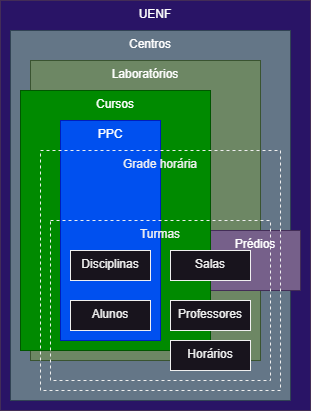
\includegraphics[width=0.5\textwidth]{files/img/2.02!3-instituicao/Diagramas Unificados-Euler-Relações entre as variáveis}
\end{MyCenteredFigure}

A \autoref{fig:relacoes} apresenta, na forma de um diagrama de Euler, a forma com a qual as variáveis presentes durante a criação da grade horária interagem entre si durante este processo. A figura, em conjunto com as descrições a seguir visam definir mais detalhadamente os termos utilizados na instituição estudada.

\begin{itemize}
  \item \textbf{Blocos/prédios}: são estruturas físicas que abrigam \textbf{salas} de aula. Cada bloco possui uma quantidade de salas, que são utilizadas para a realização das aulas;
  \item \textbf{Salas}: são estruturas físicas que abrigam as \textbf{turmas}. Cada sala possui uma capacidade máxima de \textbf{alunos}. Esse limite geralmente está atrelado à quantidade de carteiras disponíveis aos alunos, não sendo então necessariamente fixo, havendo geralmente a possibilidade de solicitar algumas carteiras de salas próximas. Elas estão teoricamente associadas aos \textbf{blocos}, visto que a compõem fisicamente, e são geridas pelos \textbf{centros}, que são responsáveis por distribuí-las. Na prática, algumas salas são preferencialmente utilizadas por determinados \textbf{cursos}, ficando então subgeridas pelos \textbf{laboratórios};
  \item \textbf{Centros}: são estruturas organizacionais que gerem os \textbf{laboratórios} e diversas \textbf{salas}. Embora cada \textbf{centro} geralmente esteja associado a um \textbf{bloco} específico, os centros não estão limitados a gerir as salas apenas deste bloco;
  \item \textbf{Laboratórios}: são estruturas organizacionais que englobam \textbf{professores}, \textbf{cursos}, \textbf{disciplinas} e \textbf{turmas}. Em sua maioria, os \textbf{laboratórios} estão associados a um único curso, entretanto, existem casos em que um laboratório está associado a mais de um curso, como é o caso do LCMAT, que está associado aos cursos de Matemática e de Ciência da Computação. Existe também o caso contrário, onde um curso está associado a mais de um laboratório, como é o do Bacharelado em Biologia que está associado a seis laboratórios;
  \item \textbf{Professores}: são aqueles que ministram as \textbf{disciplinas}. Teoricamente professor está vinculado a um \textbf{laboratório}, entretanto, na prática, os professores geralmente são associados aos \textbf{cursos} que geralmente ministram \textbf{disciplinas}. Teoricamente cada professor está passível de ministrar qualquer disciplina de seu laboratório, entretanto, na prática, os professores geralmente têm um conjunto de disciplinas que mais usualmente ministram;
  \item \textbf{Disciplinas}: um dos pontos principais na criação de uma \textbf{grade horária}. As \textbf{disciplinas} são ofertadas pelos \textbf{laboratórios} em \textbf{turmas}, que são alocadas em \textbf{salas} pelos \textbf{Centros}. Cada \textbf{PPC} define quais são as disciplinas e pré-requisitos que os \textbf{alunos} precisarão cursar. Uma mesma disciplina pode constar no PPC de diversos \textbf{cursos}. Cada disciplina possui uma carga horária, uma \textbf{ementa}, um nome e um código. Este código é composto por três letras, geralmente indicando o laboratório que o oferta, mas, em casos específicos, está associado a centros;
  \item \textbf{Turmas}: são a base da grade horária, ela consiste na representação da oferta de uma \textbf{disciplina} em um determinado \textbf{horário} e \textbf{sala}, com um determinado \textbf{professor} e para um determinado grupo de \textbf{alunos}. Mesmo que em sua maioria as disciplinas sejam ofertadas em apenas uma \textbf{turma}, existem casos em que uma disciplina é ofertada em mais de uma turma, nesses casos, um professor é atribuído como o coordenador de todas as turmas dessa disciplina. Situação essa que ocorre também com a atribuição de professores, havendo casos em que vários professores estão responsáveis por uma só turma; As turmas geralmente são direcionadas a \textbf{cursos} específicos, entretanto, existem casos em que uma turma é ofertada para mais de um curso simultaneamente;
  \item \textbf{Grade Horária}: é a representação de todas as \textbf{turmas} ofertadas em um determinado período letivo. A grade horária é composta por todas as \textbf{turmas} ofertadas, com seus respectivos \textbf{horários} e \textbf{salas}. A grade horária é a representação final do processo de criação de turmas. Esta representação geralmente é feita em formato de tabela e distribuída pelos \textbf{cursos} e \textbf{centros};
  \item \textbf{Horário}: ao se criar a \textbf{grade horária} é necessário alocar as \textbf{turmas} em um determinado momento de determinado dia da semana. Cada horário consiste de uma hora de início e uma duração (ou hora de término). Geralmente as turmas que são oferecidas aos \textbf{cursos} seguem o turno respectivo do curso, mesmo que às vezes fuja deste padrão. As turmas em sua maioria são distribuídas em horários de 2 horas com um espaço de um dia entre elas, entretanto, existem casos em que as turmas possuem 3 horas de duração. Os horários disponíveis para alocação são das 7 às 22 horas;
  \item \textbf{Cursos}: são estruturas organizacionais nos quais os \textbf{alunos} estão matriculados. Cada curso possui um turno no qual as suas turmas são ofertadas, esses turnos podem ser matutino, vespertino ou noturno;
  \item \textbf{Projeto Pedagógico do Curso (PPC)}: é o documento que define a estrutura curricular do \textbf{curso}, contendo as \textbf{disciplinas} obrigatórias, optativas e eletivas, bem como a quantidade de créditos necessários para a conclusão do curso;
  \item \textbf{Alunos}: são aqueles que frequentam as \textbf{turmas}. Cada \textbf{aluno} geralmente está vinculado ao PPC vigente para seu \textbf{curso} no ano de sua matrícula, havendo casos em que se é permitida a mudança de PPC. Segundo o PPC estão definidas quais são as \textbf{disciplinas} que o aluno deve cursar para integralizar o curso.
\end{itemize}
